\documentclass{article}

\usepackage{color}
\usepackage{graphicx}
\usepackage{tabularx}
\usepackage[frenchb]{babel}
\usepackage[utf8]{inputenc}
\usepackage[T1]{fontenc}
\usepackage{lmodern}

\usepackage{geometry,wrapfig,lipsum}
 \geometry{
 top=20mm,
 bottom=20mm,
 }
\usepackage{fancyhdr}
\pagestyle{fancy}

\renewcommand{\headrulewidth}{1pt}
\fancyhead[C]{\textbf{page \thepage}} 
\fancyhead[L]{Section : \thesection}
\fancyhead[R]{Justal k.}

\renewcommand{\footrulewidth}{1pt}
\fancyfoot[C]{\textbf{page \thepage}} 
\fancyfoot[L]{Section : \thesection}
\fancyfoot[R]{2014-2015}

\title{Hacking}
\author{Justal Kevin}
\date{30/10/2015}
\renewcommand{\contentsname}{Table des mati\`eres} 
 
\newcommand\invisiblesection[1]{%
  \refstepcounter{section}%
  \addcontentsline{toc}{section}{\protect\numberline{\thesection}#1}%
  \sectionmark{#1}} 
 
\begin{document}

\begin{center}
\textbf{\Huge{FAILLES}}\\
\line(1,0){300}\\
Verrou par verrou et l'un apr\`es l'autre, aucun syst\`eme ne r\'esistera !\\
\vspace{3cm}

\includegraphics[width=\textwidth]{0}\\
\vspace{3cm}
\textbf{\Large{JUSTAL KEVIN}}\\
2014-2015\\
\vspace{4cm}
\textbf{Justal Kevin - \color{blue}{\underline{justal.kevin@gmail.com}}}\\
\end{center}

\newpage
\tableofcontents

\newpage
\section{Ecrire des données par dessus une images - Caché du contenu}
\subsection{Prérequis}
\hspace*{0.6cm}Pour réaliser cela, il faut impérativement avoir téléchargé et installé sur son ordinateur 7zip, un utilitaire de compression.
\subsection{Etapes par Etape}
\hspace*{0.6cm}Le but ici est simplement de s'amuser à cacher des fichiers de tous genre dans une image. Cela ne semble pas avoir d'interet quelconque mais permet avec d'autres failles de faire télécharger à l'insu de l'utilisateur le malware et de le déclencher d'une autre méthode. Comment fais-t-on ?

\newpage

\section{Fonctions PHP}
\subsection{Logique humaine}
\subsubsection{L'ancrage du "str replace" ou le mauvais filtre}
\hspace*{0.6cm}Le filtre est un classique du WEB. Toutes les chaines qui entrent doivent être analysé pour empecher l'utilisateur d'entrer des choses \`a des fins malicieuses. Même ce principe de base qui consiste à simplement éliminé une chaine dans une chaine peut avec une simple erreur humaine permettre de faire un peu tout et n'importe quoi. Prenons l'exemple d'un simple formulaire :
\vspace{0.2cm}\\
\fbox{\parbox{\textwidth}{
\hspace*{0.6cm}<form method="POST" action="">\\
\hspace*{1.2cm}<input type="text" name="secret"><br>\\
\hspace*{1.2cm}<input type="submit" name="send" value="Envoyer">\\
\hspace*{0.6cm}</form>
}}
\vspace{0.2cm}\\
\hspace*{0.6cm}Il s'agit d'un simple champ texte que j'envoie par une méthode POST sur la même page que ce bout de code. Si vous ne comprenez pas,ce n'est pas bien grave, ceci ne sert qu'à mettre un contexte. Maintenant imaginons que nous souhaitons récupéré la variable et filtrer tout Javascript :
\vspace{0.2cm}\\
\fbox{\parbox{\textwidth}{
\hspace*{0.6cm}\$var=str\_replace("<script>","",\$\_POST["secret"]); 
}}
\vspace{0.2cm}\\
J'ai retrouv\'e ce bout de code sur plusieurs site et ceci m'a légèrement fait sourire. Comme on peux le voir sur cette ligne ci-dessus, nous remplaçons toutes les balises <script> par une chaine vide. Il y a pourtant ici 2 erreurs flagrantes.\\
La première demande de connaitre exactement ce que fait la balise str\_replace. Dans le HTML, il est possible d'utiliser des balises écrites en minuscule ou en majuscule. Or, str\_replace respecte la case, il m'est donc possible de rentrer une balise <SCRIPT> sans que le filtre ne s'alarme.
La deuxième est simple d'ordre logique, que se passe-t-il si j'envoie ceci via mon script PHP :
\vspace{0.2cm}\\
\fbox{\parbox{\textwidth}{
\hspace*{0.6cm}<sc<script>ript>alert("HAHA")</sc<script>ript>   
}}
\vspace{0.2cm}\\
Dans cette chaine, si nous remplaçons script par une chaine vide nous obtenons :
\vspace{0.2cm}\\
\fbox{\parbox{\textwidth}{
\hspace*{0.6cm}<script>alert("HAHA")<script> 
}}
\vspace{0.2cm}\\
 On réussit ainsi à bypasser le filtre de manière assez simple.
\subsubsection{Solutions}
	Pourquoi ne pas simplement utiliser les fonctions PHP : htmlentities() et  htmlspecialchars(). 
 
\newpage
\section{Directory transversal - Attaque sur le htaccess}
\subsection{Explications}
\subsubsection{Qu'est ce que la technologie htaccess ?}
\hspace*{0.6cm}Les fichiers .htaccess sont des fichiers de configuration de Apache. Ils permettent de s\'ecuris\'e via un mot de passe et un identifiant l'acc\'es \`a une zone du serveur. Ils sont localis\'es et ne peuvent affecter que les r\'epertoire o\`u ils r\'esident. La particularit\'e d'une telle fonctionnalit\'e apporte deux avantages. D'une part, on peux d\'el\'eguer la gestion d'une partie du site sans donner le droit de g\'erer le serveur lui-m\^eme. D'autre part, les modifications sont prises en compte sans qu'il soit n\'ecessaire de red\'emarrer le serveur HTML.

\subsubsection{Les directives htaccess}
\hspace*{0.6cm}Un fichier htaccess prend la forme suivante :
\vspace{0.2cm}\\
\fbox{\parbox{\textwidth}{
\hspace*{0.6cm}AuthUserFile /var/www/.htpasswd\\
\hspace*{0.6cm}AuthName "Visiteur, vous pénétrez dans une section réservée aux membres, veuillez vous identifier"\\
\hspace*{0.6cm}AuthType Basic\\
\hspace*{0.6cm}require Admin
}}
\vspace{0.2cm}\\
\hspace*{0.6cm}La premi\`ere directive, \textbf{AuthUserFile}, est le lien entre le htaccess et le htpasswd. Cette simple directive indique simplement o\`u se situe le fichier htpasswd. Le chemin inscrit ici est g\'en\'eralement le chemin d'acc\`es absolue mais il est possible de trouver aussi un chemin relative mais cela reste tout de m\^eme relativement rare.
\vspace{0.2cm}\\
La directive \textbf{AuthName} permet de sp\'ecifier un titre \`a la fen\^etre de connexion.
\vspace{0.2cm}\\
\hspace*{0.6cm}La directive \textbf{AuthType} indique le type d'authentification. Il n'existe que deux types possibles : Basic ou Digest. Le premier type indique simplement que le mot de passe lors de l'authentification sera transmise en clair du client au serveur. C'est pourquoi cette m\'ethode n'est pas \`a utiliser pour un transfert de donn\'ee sensible. Le type Digest est un sois-disant type am\'eliorant la s\'ecurit\'e du transfert, cependant de nombreuses failles existent ici. Ce qui rend ce type inutile car plus lourd \`a mettre en place et pas vraiment s\'ecuris\'e.
\vspace{0.2cm}\\
La directive \textbf{requiere} sp\'ecifie simplement qui est autoris\'e \`a acc\'eder \`a cette partie du site. On ira donc chercher dans le fichier htpasswd l'utilisateur Admin pour comparer le mot de passe.
\subsubsection{Les directives htpasswd}
\hspace*{0.6cm}Un fichier htpasswd prend la forme suivante :
\vspace{0.2cm}\\
\fbox{\parbox{\textwidth}{
\hspace*{0.6cm}admin1:\$apr1\$Ikl22aeJ\$w1uWlBGlbatPnETT2XGx.. \\
\hspace*{0.6cm}admin2:\$apr1\$yJnQGpTi\$WF5eCC/8lKsgBKY7fvag60 
}}
\vspace{0.2cm}\\
\hspace*{0.6cm}Un fichier httpasswd prend toujours la forme ci-dessus. Ce fichier lie un utilisateur \`a un password crypt\'e via un algorithme comme SHA, DES, MD5...

\subsection{La navigation transversale ou Directory transversal}
\hspace*{0.6cm}Pour expliqu\'e la faille, je prendrais un exemple. Le site w3challs.com dispose d'un exemple sur cette faille du syst\`eme. Avant m\^eme de commencer l'exp\'erimentation, il faut encore un peu d'explication pour comprendre la faille. Cette faille r\'eside dans le PHP du site et en particulier dans la balise include.
\vspace{0.2cm}\\
\fbox{\parbox{\textwidth}{
\hspace*{0.6cm}\$template = 'red.php';\\
\hspace*{0.6cm}if (isset(\$\_COOKIE['TEMPLATE']))\\
\hspace*{1.2cm}\$template = \$\_COOKIE['TEMPLATE'];\\
\hspace*{0.6cm}include ("/home/users/phpguru/templates/" . \$template);
}}
\vspace{0.2cm}\\
\hspace*{0.6cm}Ici, le fait que dans l'include, on ne v\'erifie pas que le r\'esultat attendu soit une page .html ou .php, on peux alors imaginer de modifi\'e la variable \$template. Il y a plusieurs mani\`eres de proc\'ed\'e qui d\'ependent de la mani\`ere dont est impl\'ement\'e le code du site que l'on souhaite attaquer : Par l'URL, Par la requ\`ete HTML...\\
\hspace*{0.6cm}Dans le cas ci-dessus, on utilise \$\_COOKIE, on en retient donc que la page ou la destination vers o\`u pointe \$template a \'et\'e enregistr\'e sur l'ordinateur de l'utilisateur. Il est donc possible de modifier la requ\`ete avant de l'envoyer au serveur.
\vspace{0.2cm}\\
Imaginons alors que la variable template soit "../../../.htaccess", on remonte alors les repertoires jusqu'au root. Si le systeme de la machine est Linux, il existe alors forcement un repertoire etc/passwd. Maintenant, sur les serveur en ligne, les developpeurs posent g\'en\'eralement ces dossiers dans des repertoires comme admin/.htaccess ou encore pass/.htaccess. Il suffit de faire preuve d'un peu d'imagination pour trouver o\`u pourrait se trouver le fichier.

\subsection{Exploitation}
\hspace*{0.6cm}Sur w3chall.com, on trouve une page avec cette faille. La premi\`ere chose \`a faire est donc de chercher le fichier .htaccess. En forcant, on trouve que le fichier assez rapidement. Dans la barre d'adresse, il suffit de finir l'adresse par :
\vspace{0.2cm}\\
\fbox{\parbox{\textwidth}{
\hspace*{0.6cm}/?page=../admin/.htaccess
}}
\vspace{0.2cm}\\
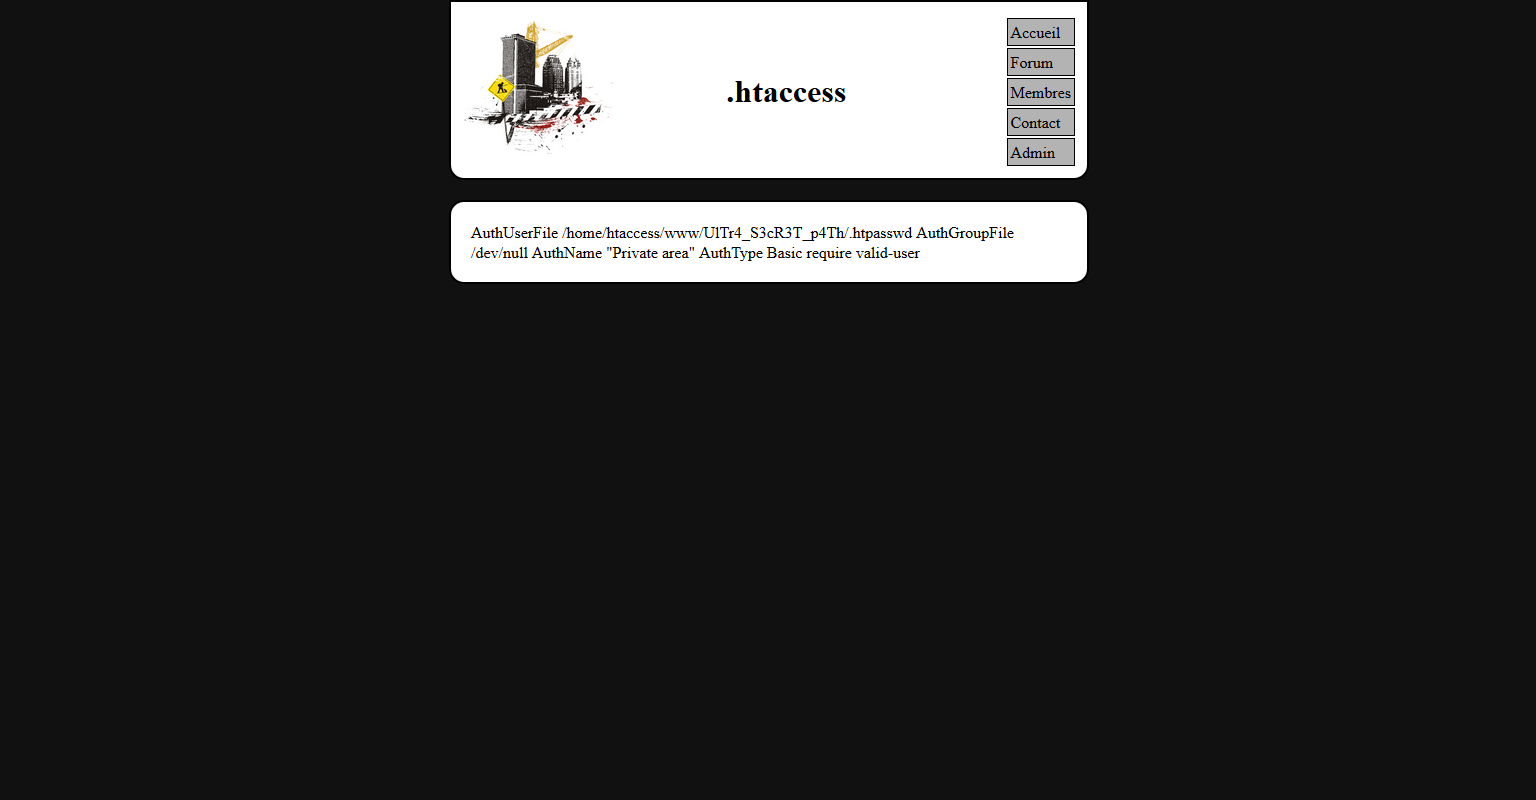
\includegraphics[width=\textwidth]{2}\\
\vspace{0.2cm}\\
Bien entendu, avant d'arriver \`a cela, j'ai tap\'e plusieurs autres chemins comme ./admin/.htaccess ou encore .htaccess. Une fois ici, on remarque la g\'en\'erosit\'e du syst\`eme qui nous donne l'emplacement exacte du fichier htpasswd. Il suffit alors de s'y rendre :
\vspace{0.2cm}\\
\fbox{\parbox{\textwidth}{
\hspace*{0.6cm}?page=../UlTr4\_S3cR3T\_p4Th/.htpasswd
}}
\vspace{0.2cm}\\
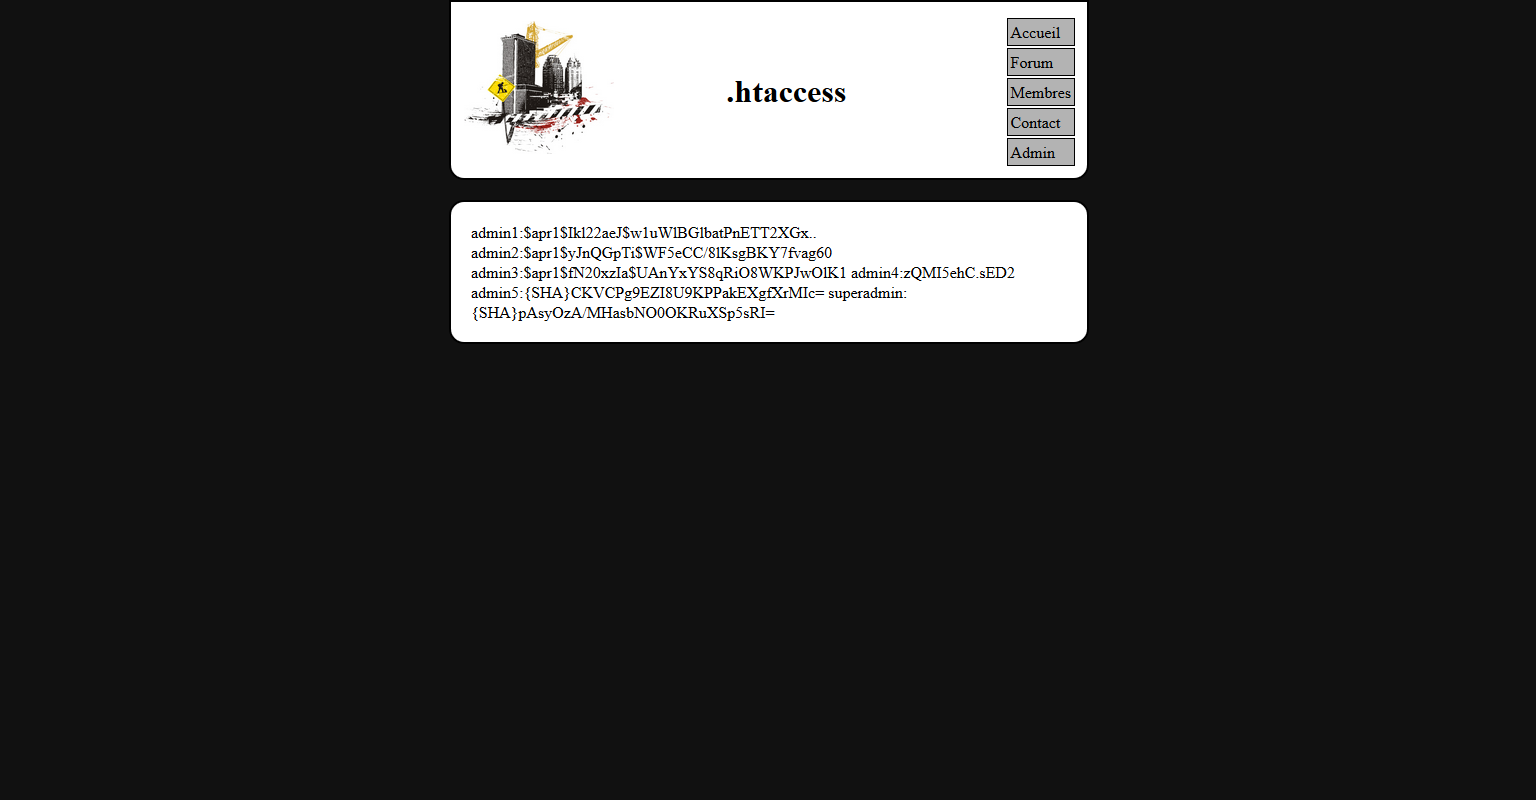
\includegraphics[width=\textwidth]{3}\\
\vspace{0.2cm}\\
\hspace*{0.6cm}Et voila qu'apparaisent sous vos yeux les passwords et logins qui se trouvent dans le fichier htpasswd. Ils sont bien entendu crypté mais avec l'utilisation d'un logiciel tiers comme John the Ripper, la reconstitution du password d'origine n'est qu'une question de temps.
\subsection{Variante}
\hspace*{0.6cm}La premi\`ere correstion apport\'e par les d\'eveloppeurs furent d'ajouter l'extension du fichier \`a la fin de l'include. Ce qui donnait un lien finissant toujours par .html ou .php. Il devient alors th\'eoriquement impossible de rentrer quelques choses finissant par aucune extension comme nous l'avons fait jusqu'\`a maintenant. Erreur ! Il est possible de terminer une chaine \`a l'endroit o\`u l'on souhaite en ajoutant le charat\`ere de fin de chaine : le null ou encore \%00. Ce qui dans notre cas donnerais :
\vspace{0.2cm}\\
\fbox{\parbox{\textwidth}{
\hspace*{0.6cm}/?page=../admin/.htaccess\%00.html
}}
\vspace{0cm}\\
Cependant le serveur ne lira cette chaine que jusqu'au charatere null, le reste sera ignor\'e.
\subsection{Solutions}
Pour se pr\'emunir d'une telle attaque, pourquoi ne pas simplement escape tout les ../ ou \%2e\%2e/ (si encod\'e) lors des navigations.

\newpage
\section{SMTP Injection - Injection dans la fonction php mail()}
\subsubsection{Qu'est ce qu'un envoie de message ?}
L'envoie de message sur le web se traduit par l'utilisation du protocole SMTP. La communication entre le client et le serveur qui va recueillir le message est la suivante :
\vspace{0.2cm}\\
\fbox{\parbox{\textwidth}{
S: 220 smtp.example.com ESMTP Postfix
\vspace{0.2cm}\\
C: HELO relay.example.org 
\vspace{0.2cm}\\
S: 250 Hello relay.example.org, I am glad to meet you
\vspace{0.2cm}\\
C: MAIL FROM:<bob@example.org>
\vspace{0.2cm}\\
S: 250 Ok
\vspace{0.2cm}\\
C: RCPT TO:<alice@example.com>
\vspace{0.2cm}\\
S: 250 Ok
\vspace{0.2cm}\\
C: RCPT TO:<theboss@example.com>
\vspace{0.2cm}\\
S: 250 Ok
\vspace{0.2cm}\\
C: DATA
\vspace{0.2cm}\\
S: 354 End data with <CR><LF>.<CR><LF>
\vspace{0.2cm}\\
\color{blue}{C: From: "Bob Example" <bob@example.org>\\
C: To: "Alice Example" <alice@example.com>\\
C: Cc: theboss@example.com\\
C: Date: Tue, 15 January 2008 16:02:43 -0500\\
C: Subject: Test message\\
C: \vspace{0.0cm}\\
C: Hello Alice.
C: This is a test message with 5 header fields and 4 lines in the message body.\\
C: Your friend,\\
C: Bob\\
C: .}
\vspace{0.2cm}\\
\color{black}{S: 250 Ok: queued as 12345
\vspace{0.2cm}\\
C: QUIT
\vspace{0.2cm}\\
S: 221 Bye\\
{The server closes the connection}}
}}
\vspace{0.2cm}

Nous n'allons pas nous interessé à tous le concept entre le client et le serveur (bien que cela tout aussi intéressant). La partie en bleu est la seule utile pour comprendre la faille. Comme on peux le voir, on retrouve ici toutes les informations composants un email.

\subsubsection{La fonction mail() de php}

Dans PHP, il existe une méthode pour envoyer un mail assez facile à utiliser. Comme on peux le voir ci-dessous, on retrouve la variable pour le destinataire, la variable pour le sujet du mail, la variable pour le corp du message et une variable pour les headers du mail. Cette dernière variable est celle qui nous intéresse le plus et c'est sur cette dernière que je vais agir.
\vspace{0.2cm}\\
\fbox{\parbox{\textwidth}{
\hspace*{0.6cm}mail(\$destinataire, \$sujet, \$message, \$headers);
}}
\vspace{0cm}\\
La variable header permet entre autre de rajouter un élément pour le mail. Dans le code en bleu précédemment, on retrouvait CC par exemple. Ci-dessous, je fais une liste des différents Header que l'on peux utiliser (non-exhaustive) :\\
\begin{itemize}
  \item CC (Pour mettre quelqu'un en copie du message)
  \item BCC (Pour mettre quelqu'un en copie du message de manière invisible)
  \item FCC (Pour copier le message dans un fichier)
  \item Reply-To (L'adresse vers où diriger le message si le destinataire répond)
\end{itemize}

\subsection{Qu'est ce qu'une injection de header}

Lorsque l'on envoie un mail par la fonction mail() de php, l'envoie se tranformera en ceci lors de la requête :\\
\fbox{\parbox{\textwidth}{
\hspace*{0.6cm}To: \$destinataire\\
\hspace*{0.6cm}Subject: \$sujet\\
\hspace*{0.6cm}\$headers\\
\hspace*{0.6cm}\$message
}}
\vspace{0.1cm}\\

Dans cette fonction, de nombreux filtres existent sur les varaibles \$destinataire, \$subject et \$message. Cependant sur le champs \$header, il est toujours possible d'agir et il le sera certainement toujours. Maintenant, il faut comprendre maintenant comment ce bout de texte est envoyé au serveur, ce n'est pas aussi beau qu'au dessus. Ces informations sont séparé par des <LF> afin que le serveur puissent différencier les différentes champs. Un <LF> est un passage à la ligne dont la traduction hexadécimale est 0x0A. Cette information est très importante. Le but de la faille va être de surcharger le header avec des informations complémentaire pour obtenir par exemple une copie du message. Par exemple, si notre message est le suivant :\\
\fbox{\parbox{\textwidth}{
\hspace*{0.6cm}mail("lala@gmail.com", "Lala", "LalaLALA", "");
}}
\vspace{0.1cm}\\

Cela se traduit par :\\
\fbox{\parbox{\textwidth}{
\hspace*{0.6cm}To: lala@gmail.com\\
\hspace*{0.6cm}Subject: Lala\\
\hspace*{0.6cm}\\
\hspace*{0.6cm}LalaLALA
}}
\vspace{0.1cm}\\

Maintenant, si l'on change le header par quelques choses comme ceci : \%0ABCC:lolo@gmail.com\\
\fbox{\parbox{\textwidth}{
\hspace*{0.6cm}To: lala@gmail.com\\
\hspace*{0.6cm}Subject: Lala\\
\hspace*{0.6cm}\\
\hspace*{0.6cm}BCC:lolo@gmail.com\\
\hspace*{0.6cm}LalaLALA
}}
\vspace{0.1cm}\\

On se retrouve alors à injecter un header qui n'était pas prévu à la base !

\subsection{Exemple}

Pour expliquer la faille, je vais me servir du site de w3Challs. Sur ce dernier, il y a une page pour tester ce type d'injection. Pour commencer, il faut chercher un champ d'un formulaire qui pourrait utiliser cette fonction.
\vspace{0.2cm}\\
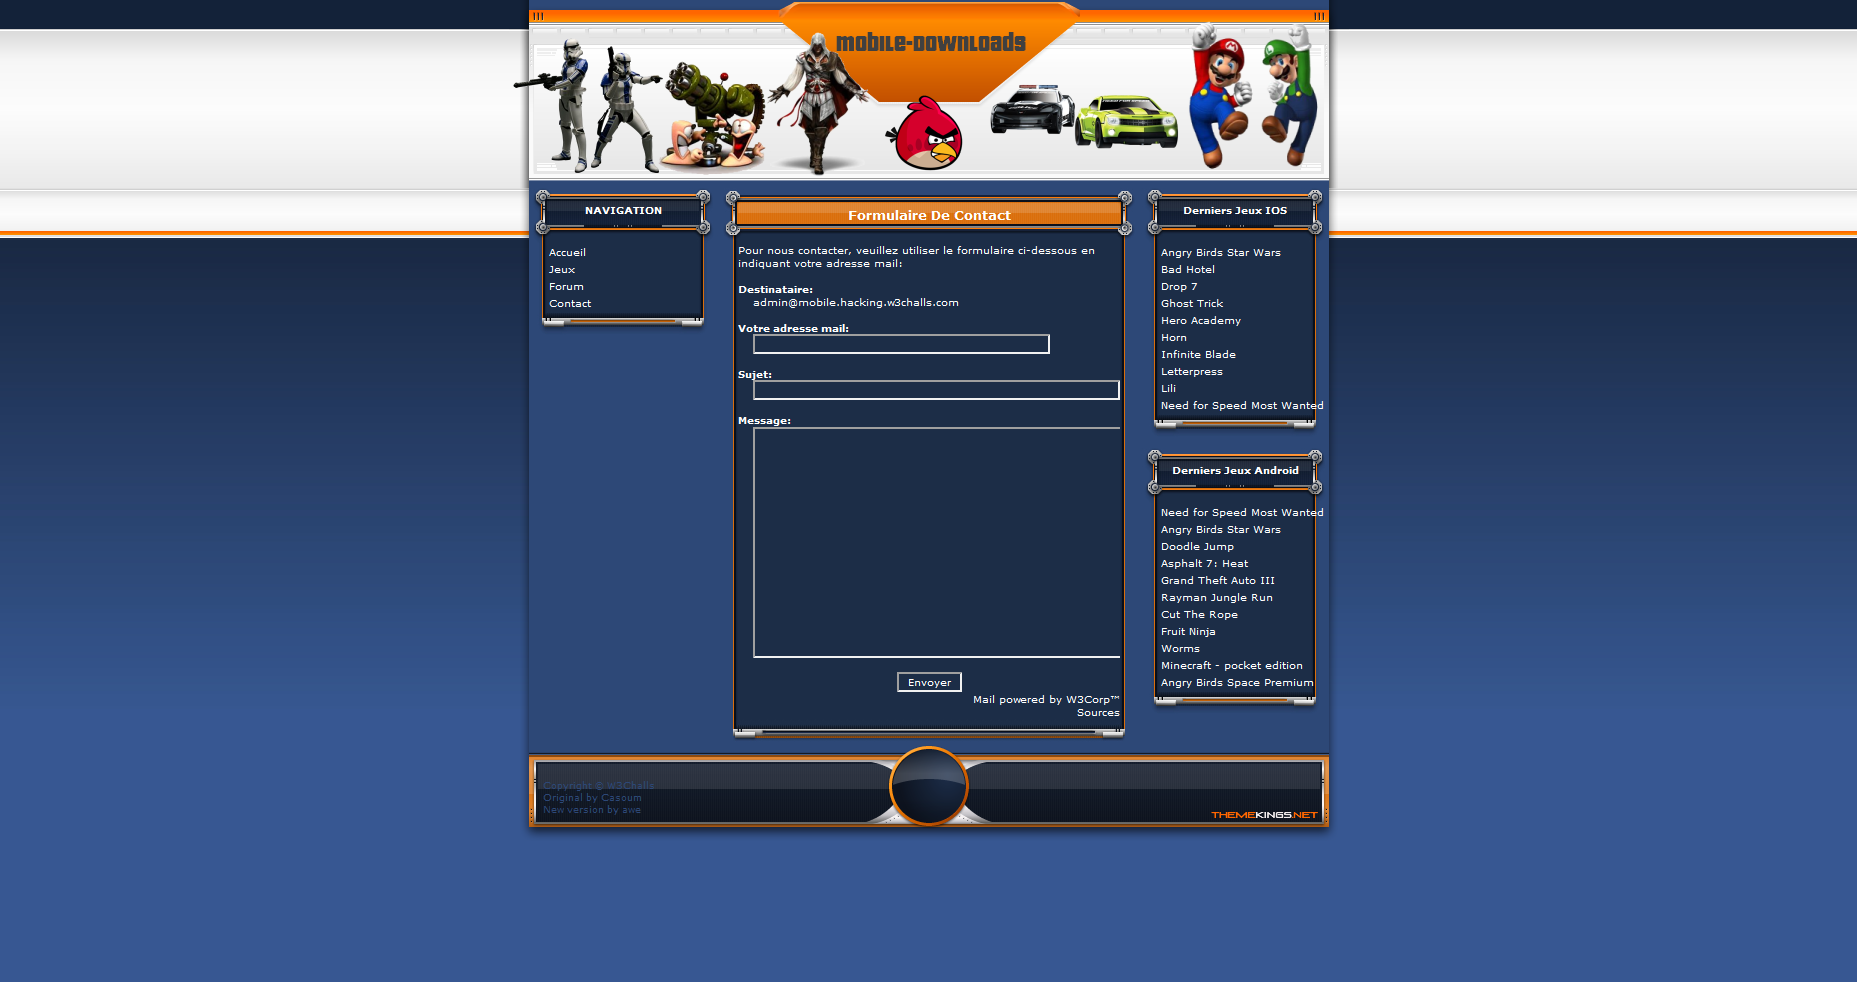
\includegraphics[width=\textwidth]{8}\\
\vspace{0.2cm}

On trouve alors un très beau (et surtout moche) formulaire pour envoyer des messages aux créateurs du site. On remarque que le premier champ est très susceptible d'avoir une faille. On tente donc une injection de header. Je vais dans un premier temps créer ma petite injection dans le champ adresse mail en écrivant ceci : lala@gmail\%0ABCC:lolo@gmail.com
\vspace{0.2cm}\\
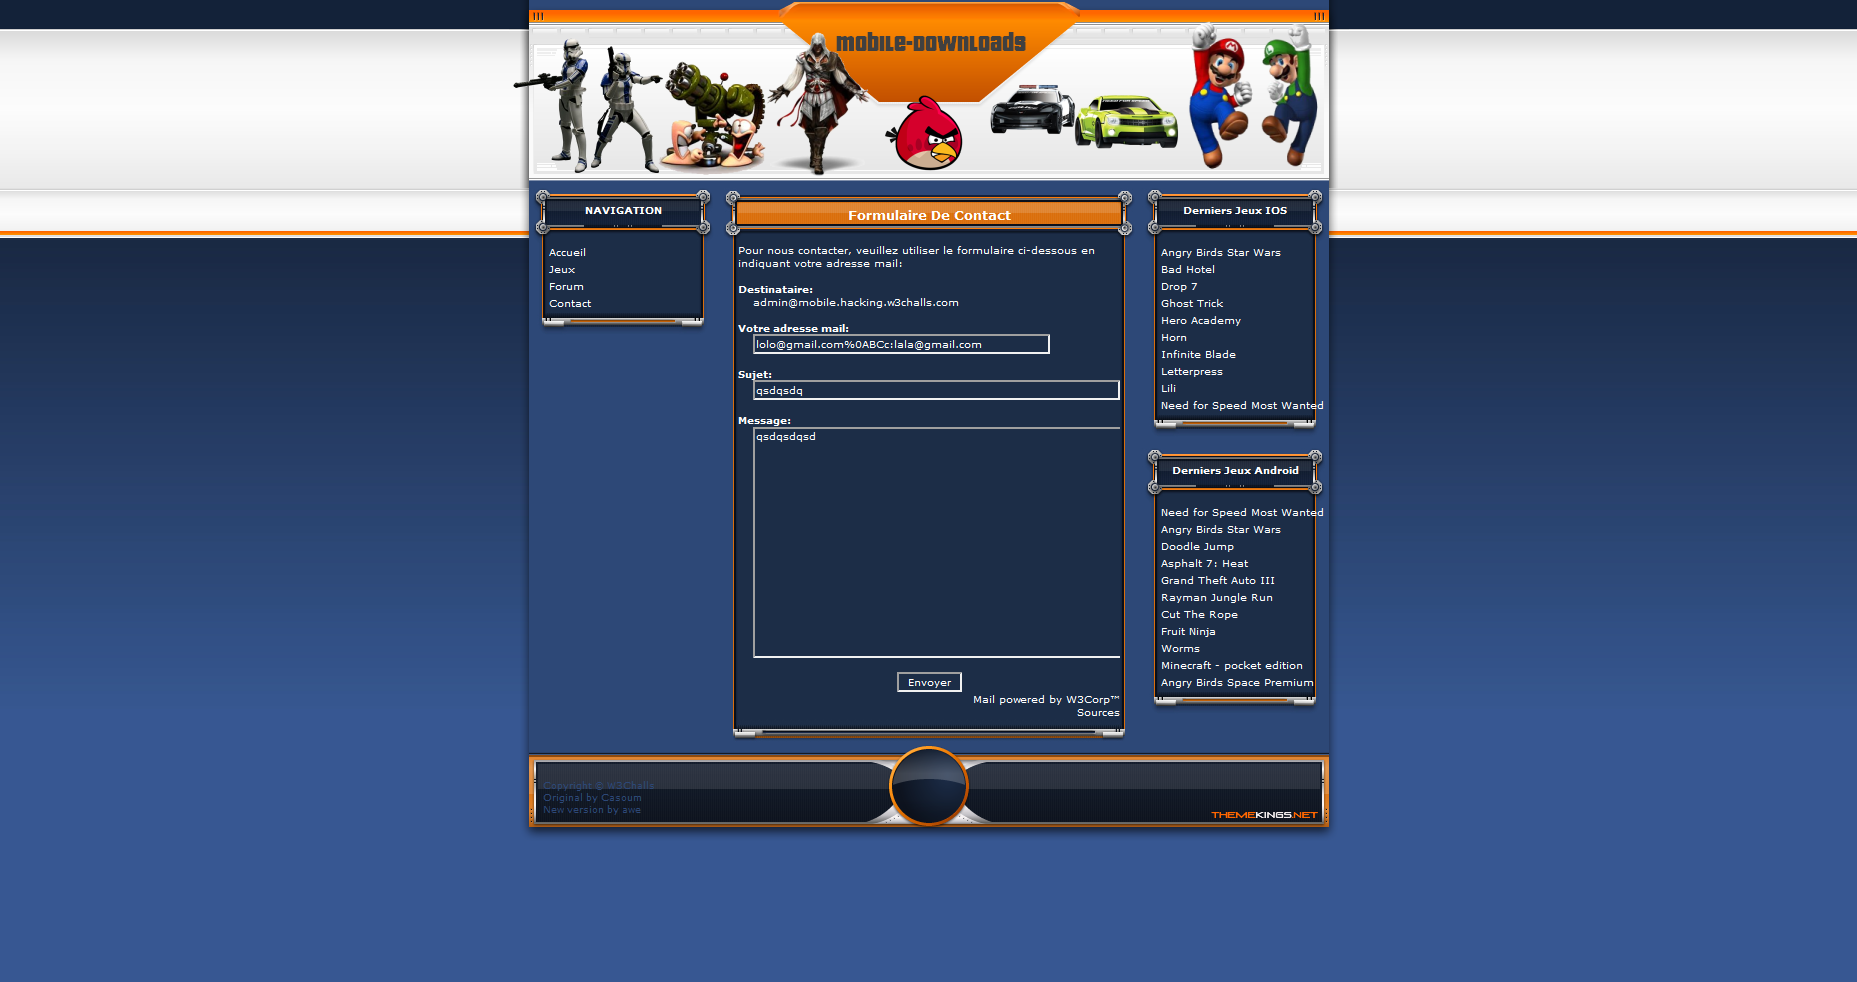
\includegraphics[width=\textwidth]{9}\\
\vspace{0.2cm}

En utilisant ensuite Tamper Data afin d'altérer la requête POST, on peux prévenir notre requête d'être encoder en format URL. Car dans notre cas, le symbole \% est automatiquement transformé par Firefox en \%25, ce qui n'est pas ce que l'on veut.
\vspace{0.2cm}\\
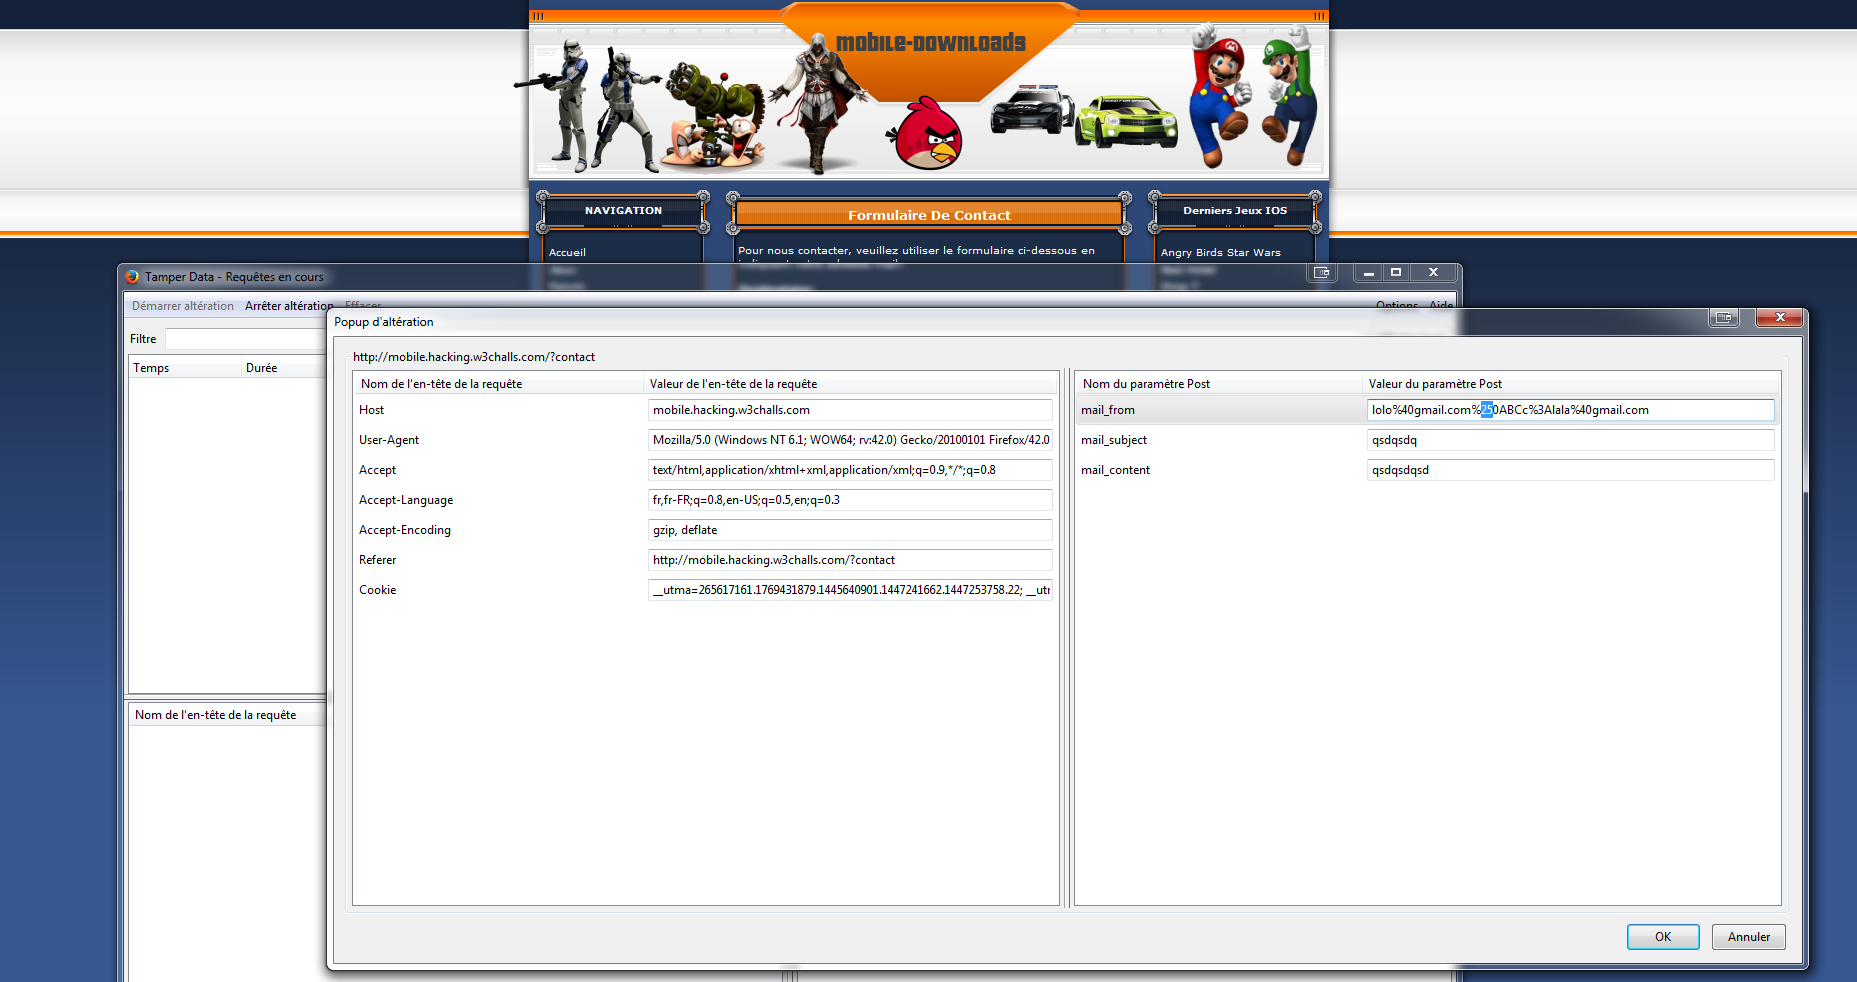
\includegraphics[width=\textwidth]{10}\\
\vspace{0.2cm}

Enfin, on envoie la requête et pouvons maintenant consulter sur notre adresse un double du mail que l'admin a reçu :p Avec cette méthode, il est possible de spammer des personnes, de se faire passer pour certaines personnes...

\subsection{Solutions}
Pour se protéger contre ce type d'attaque, il suffit de vérifier que les informations entré par l'utilisateur ne contiennent pas les symboles \textbackslash n ou \textbackslash r. Par exemple, le bout de code suivant réalise cette opération :\\
\vspace{0.1cm}\\
\fbox{\parbox{\textwidth}{
\hspace*{0.6cm}if(eregi("\textbackslash r",\$from) or eregi("\textbackslash n",\$from)) \{\\
\hspace*{1.2cm}die("Why ?? :(");\\
\hspace*{0.6cm}\}
}}
\vspace{0.1cm}\\

\newpage
\section{Attaque temporel - Attaque par Canaux cachés}
\subsection{Qu'est ce qu'un canal caché ?}

\newpage
\section{CSRF - Cross-site request forgery}
\subsection{Qu'est ce qu'une attaque CRSF ?}
Pour expliquer cela, il est beaucoup plus intéressant de prendre un exemple. Imaginons la scène suivante :\\
\begin{itemize}
\item Une personne s'enregistre à sa banque normalement\\
\item La banque donne un cookie a cette personne qui permet de définir session\\
 (Set-Cookie: SESSIONID=a804696f-93fc-48cf-9b02-267d9ed773c0)\\
\item Puis sur d'autre onglet, cette personne navigue sur d'autres sites\\
\item Et tombe sur un site, avec un code malicieux :\\
\fbox{\parbox{\textwidth}{
\begin{scriptsize}
<form name="attack" enctype="text/plain" action="https://bank.example.com/api/transfer" METHOD="POST">\\
  <input type="hidden" name='{"from": "Savings", "to": "00302319550440", "amount": "100.00"}'>\\
</form>\\
<script>document.attack.submit();</script>
\end{scriptsize}
}}\\
\item Lorsque l'utilisateur arrive sur la page, son navigateur lit la page et va exécuter le code. Ce qui va résulter à un transfert de 100 euros à un certain compte bancaire\\
\item Comme l'utilisateur a un cookie avec une session valide, la requête émis via le formulaire va etre accepté par le site de la banque
\end{itemize}

\newpage
\section{XSS}
\subsection{XSS Test}
Pour testé rapidement si une faille XSS est possible à un endroit ou non, on peux utiliser des chaines de test telles que les suivantes :
\vspace{0.2cm}\\
\fbox{\parbox{\textwidth}{
\vspace{0.2cm}';alert(String.fromCharCode(88,83,83))//';alert(String.fromCharCode(88,83,83))//";\\
alert(String.fromCharCode(88,83,83))//";alert(String.fromCharCode(88,83,83))//--\\
></SCRIPT>">'><SCRIPT>alert(String.fromCharCode(88,83,83))</SCRIPT>
\vspace{0.2cm}
}}
\vspace{0.2cm}

ou encore une balise déprécié :
\vspace{0.2cm}\\
\fbox{\parbox{\textwidth}{
\vspace{0.2cm}
<PLAINTEXT>
\vspace{0.2cm}
}}
\vspace{0.2cm}

Ou encore une autre version si l'espace est limité par le nombre de caractères, il faut cependant pour cette dernière analysé le code source retourné et chercher ceci " <XSS" ou "\&lt;XSS" :
\vspace{0.2cm}\\
\fbox{\parbox{\textwidth}{
\vspace{0.2cm}
'';!--"<XSS>=\&\{()\}
\vspace{0.2cm}
}}
\vspace{0.2cm}\\

\subsection{Simple XSS - balise script}
Prenons le script suivant sans aucune protection :
\vspace{0.2cm}\\
\fbox{\parbox{\textwidth}{
\vspace{0.2cm}
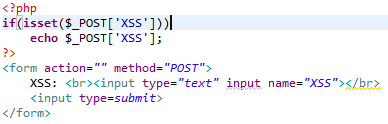
\includegraphics[width=0.5\textwidth]{12}
\vspace{0.2cm}
}}
\vspace{0.2cm}\\
Ici la moindre attaque XSS est possible, il est possible d'écrire directement du code dans les balises scripts. Par exemple, <script>alert(1)</script> :
\vspace{0.2cm}\\
\fbox{\parbox{\textwidth}{
\vspace{0.2cm}
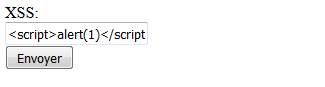
\includegraphics[width=0.4\textwidth]{13}
\vspace{0.2cm}
}}
\vspace{0.2cm}\\
On obtient alors le résultat suivant qui nous montre qu'une faille XSS est possible ici :
\vspace{0.2cm}\\
\fbox{\parbox{\textwidth}{
\vspace{0.2cm}
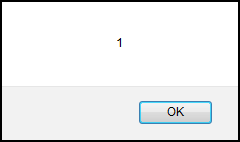
\includegraphics[width=0.5\textwidth]{14}
\vspace{0.2cm}
}}
\subsection{XSS Trick - Bypass htmlspecialchars in some cases}
Dans certains cas, la fonction htmlspecialchars est inutile comme on peux le voir ci-dessous :
\vspace{0.2cm}\\
\fbox{\parbox{\textwidth}{
\vspace{0.2cm}
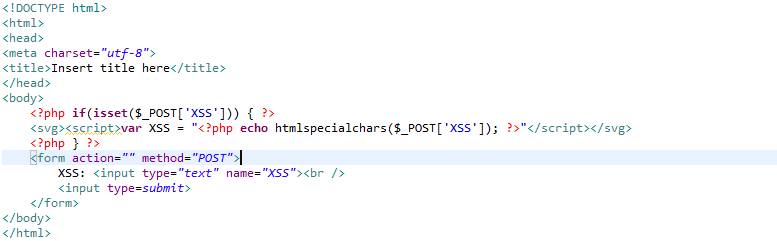
\includegraphics[width=0.9\textwidth]{15}
\vspace{0.2cm}
}}
\vspace{0.2cm}\\
On peux alors faire notre injection de la manière suivante : xss";prompt(/XSS/);//
\vspace{0.2cm}\\
\fbox{\parbox{\textwidth}{
\vspace{0.2cm}
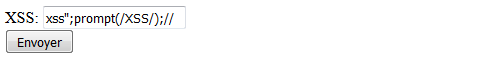
\includegraphics[width=0.5\textwidth]{16}
\vspace{0.2cm}
}}
\vspace{0.2cm}\\
On obtient alors le résultat suivant qui nous montre qu'une faille XSS est possible ici :
\vspace{0.2cm}\\
\fbox{\parbox{\textwidth}{
\vspace{0.2cm}
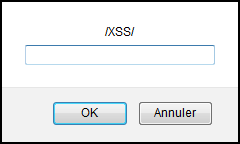
\includegraphics[width=0.5\textwidth]{17}
\vspace{0.2cm}
}}
\subsection{XSS - Bypass htmlspecialchars et htmlentities avec simples guillemets}
Si on se réfère à la documentation de PHP, par défaut sur la fonction htmlentites et/ou htmlspecialchars le flag ENT\_COMPAT est utilisé dans la fonction. Ce flag signifie que la fonction convertit les guillements doubles et ignore les guillemets simples. Autrement dit, si le codeur en question a écrit une fonction comme :
\vspace{0.2cm}\\
\fbox{\parbox{\textwidth}{
\vspace{0.2cm}
echo {\color{red}'}<a href={\color{blue}"}{\color{red}'}.htmlspecialchars(\$\_POST['XSS']).{\color{red}'}{\color{blue}"}>Test</a><br />{\color{red}'};
\vspace{0.2cm}
}}
\vspace{0.2cm}

Si on regarde attentivement, une injection XSS est donc ici possible avec par exemple la saisie suivante :
\vspace{0.2cm}\\
\fbox{\parbox{\textwidth}{
\vspace{0.2cm}
XSS' autofocus onfocus='alert(1)
\vspace{0.2cm}
}}
\vspace{0.2cm}

L'autofocus permet de mettre automatiquement le focus sur le lien dès le chargement de la page tandis que le onfocus sera la fonction appelé dès que le lien aura le focus. Autrement dit, la fonction à l'intérieur du onfocus sera automatiquement chargé au chargement de la page sur le PC du client.

Effectuons un petit test avec onmouseover pour voir le résultat cela dans un navigateur récent :
\vspace{0.2cm}\\
\fbox{\parbox{\textwidth}{
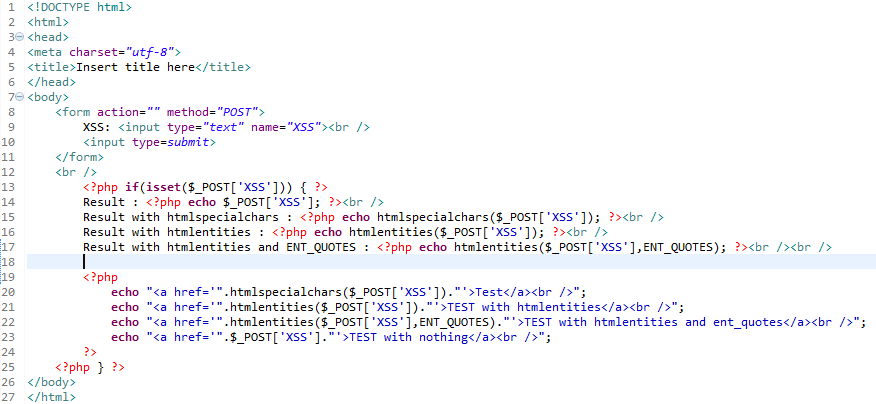
\includegraphics[width=\textwidth]{18}
}}
\vspace{0.2cm}

Je vais aussi utilisé Data Temper, un plugin de firefox, pour altérer ma requête POST afin de bypasser l'encodage du navigateur.
\vspace{0.2cm}\\
\fbox{\parbox{\textwidth}{
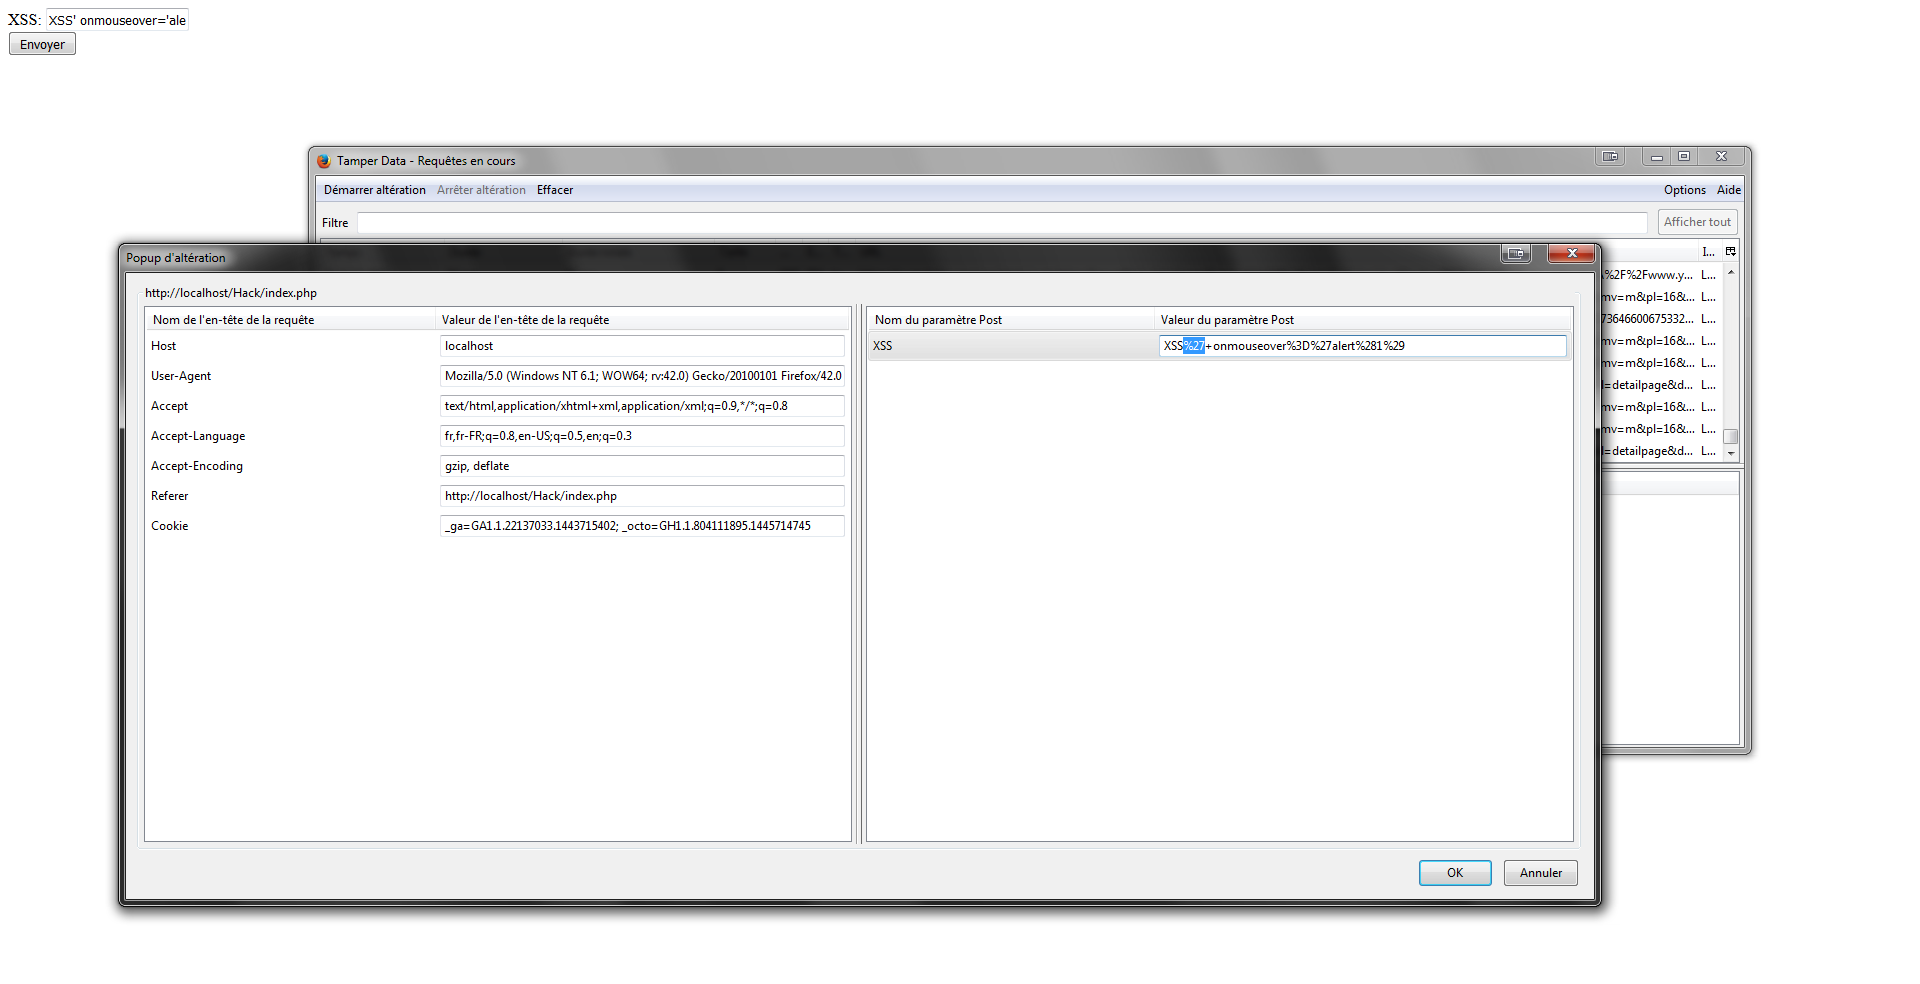
\includegraphics[width=\textwidth]{19}
}}
\vspace{0.2cm}

On obtient alors le résultat suivant :
\vspace{0.2cm}\\
\fbox{\parbox{\textwidth}{
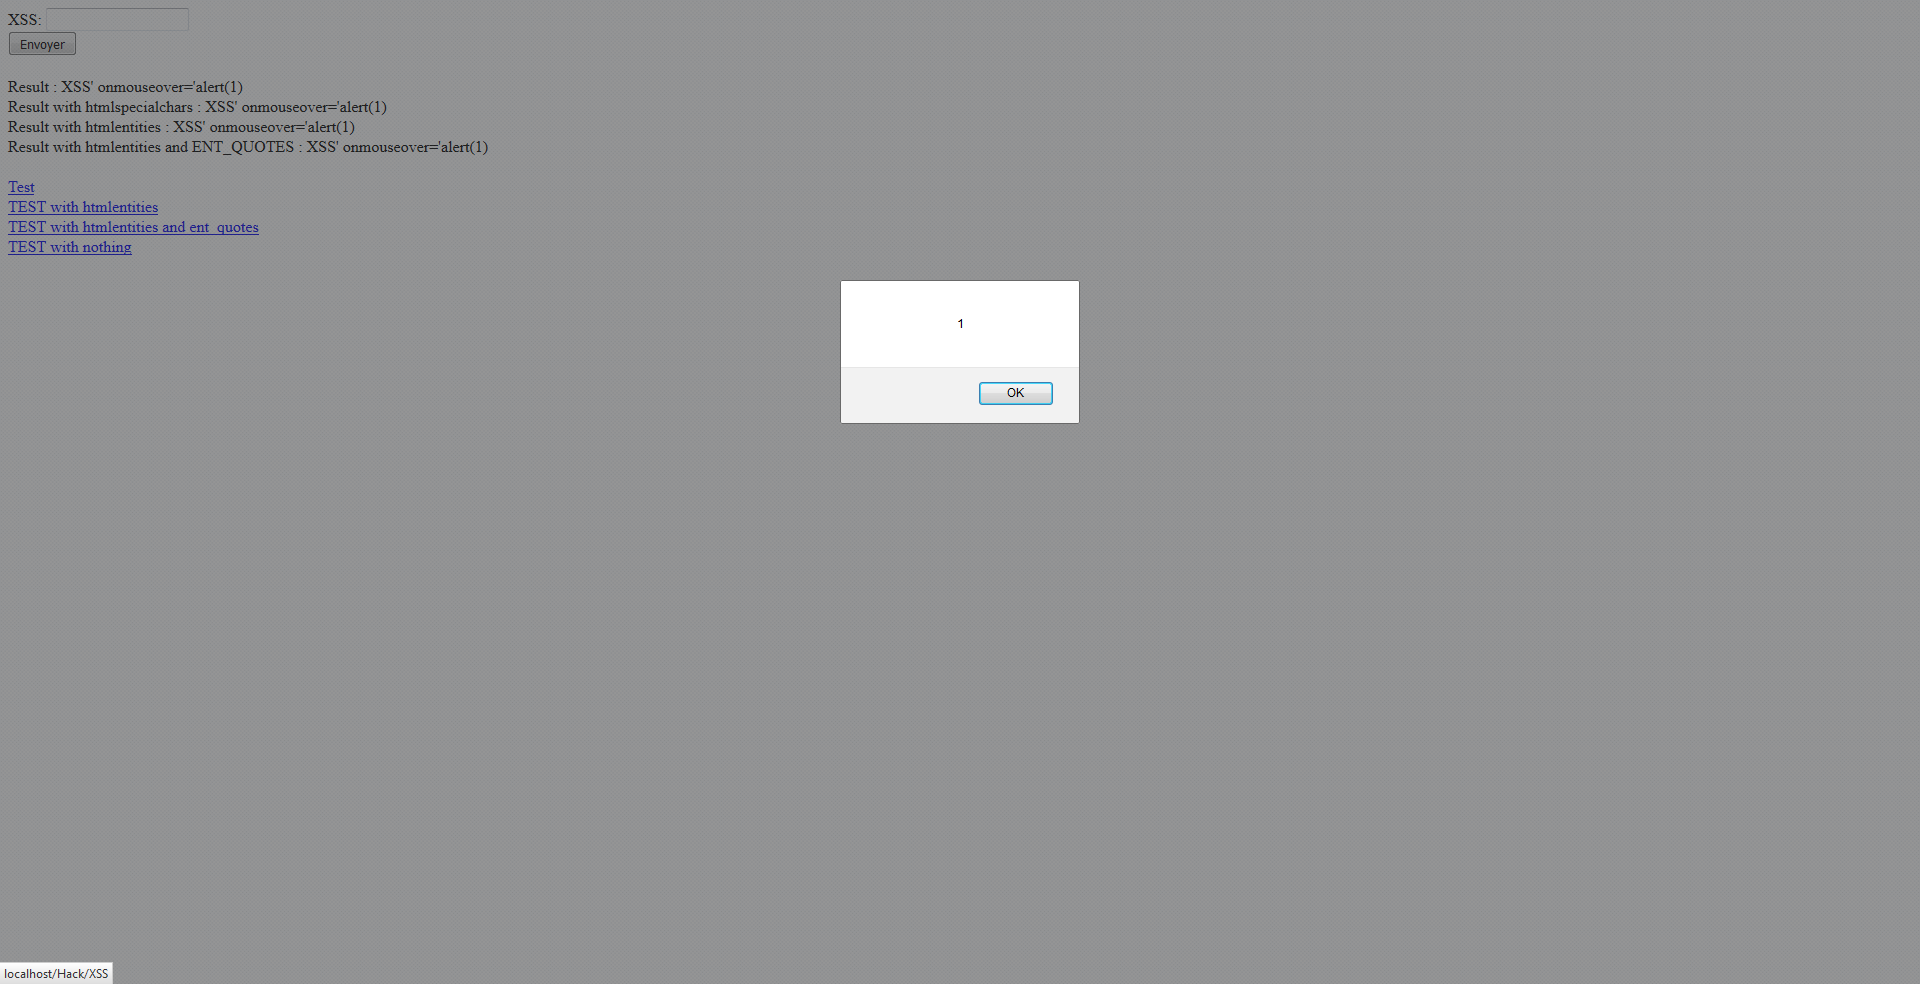
\includegraphics[width=\textwidth]{20}
}}
\vspace{0.2cm}
\subsection{XSS - Bypass htmlspecialchars et htmlentities avec espace}

Dans la continuité du chapitre précédent, j'ai rencontré de nombreux code sur internet qui ressemblait à ceci afin de par exemple pré remplir un champ :
\vspace{0.2cm}\\
\fbox{\parbox{\textwidth}{
echo "<input value={\color{blue}"}.htmlspecialchars(\$\_POST['XSS']).{\color{blue}"}>";
}}
\vspace{0.2cm}
Encore une fois, il est possible ici de reproduire une injection XSS comme précédemment. Par exemple, une injection comme celle-ci :
\vspace{0.2cm}\\
\fbox{\parbox{\textwidth}{
XSS autofocus onfocus=alert(1)
}}
\vspace{0.2cm}
Les espaces feront que le champ value sera égale à XSS puis l'autofocus et onfocus seront donc des éléments de la balise. De la même manière que précédemment, l'autofocus permettra d'exécuter automatiquement le script situé dans le champ onfocus. On s'affranchit ainsi de la restriction de la balise.

Effectuons un petit exemple avec la fonction onmouseover :
\vspace{0.2cm}\\
\fbox{\parbox{\textwidth}{
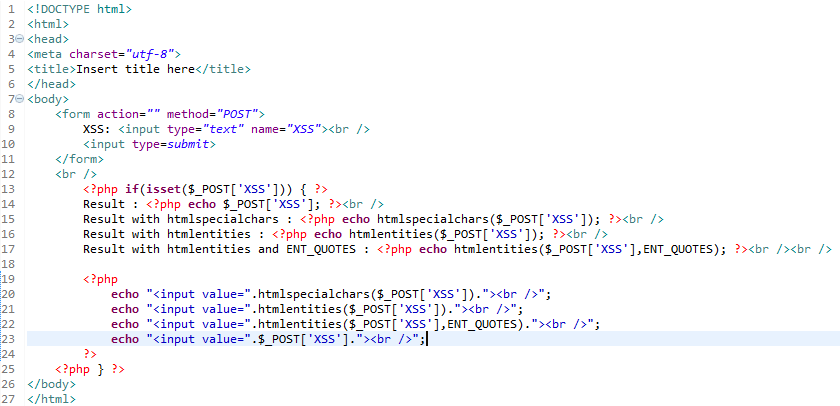
\includegraphics[width=\textwidth]{21}
}}
\vspace{0.2cm}

Cette fois, il n'y a pas besoin d'effectuer un quelconque tamper sur les données, on obtient donc :
\vspace{0.2cm}\\
\fbox{\parbox{\textwidth}{
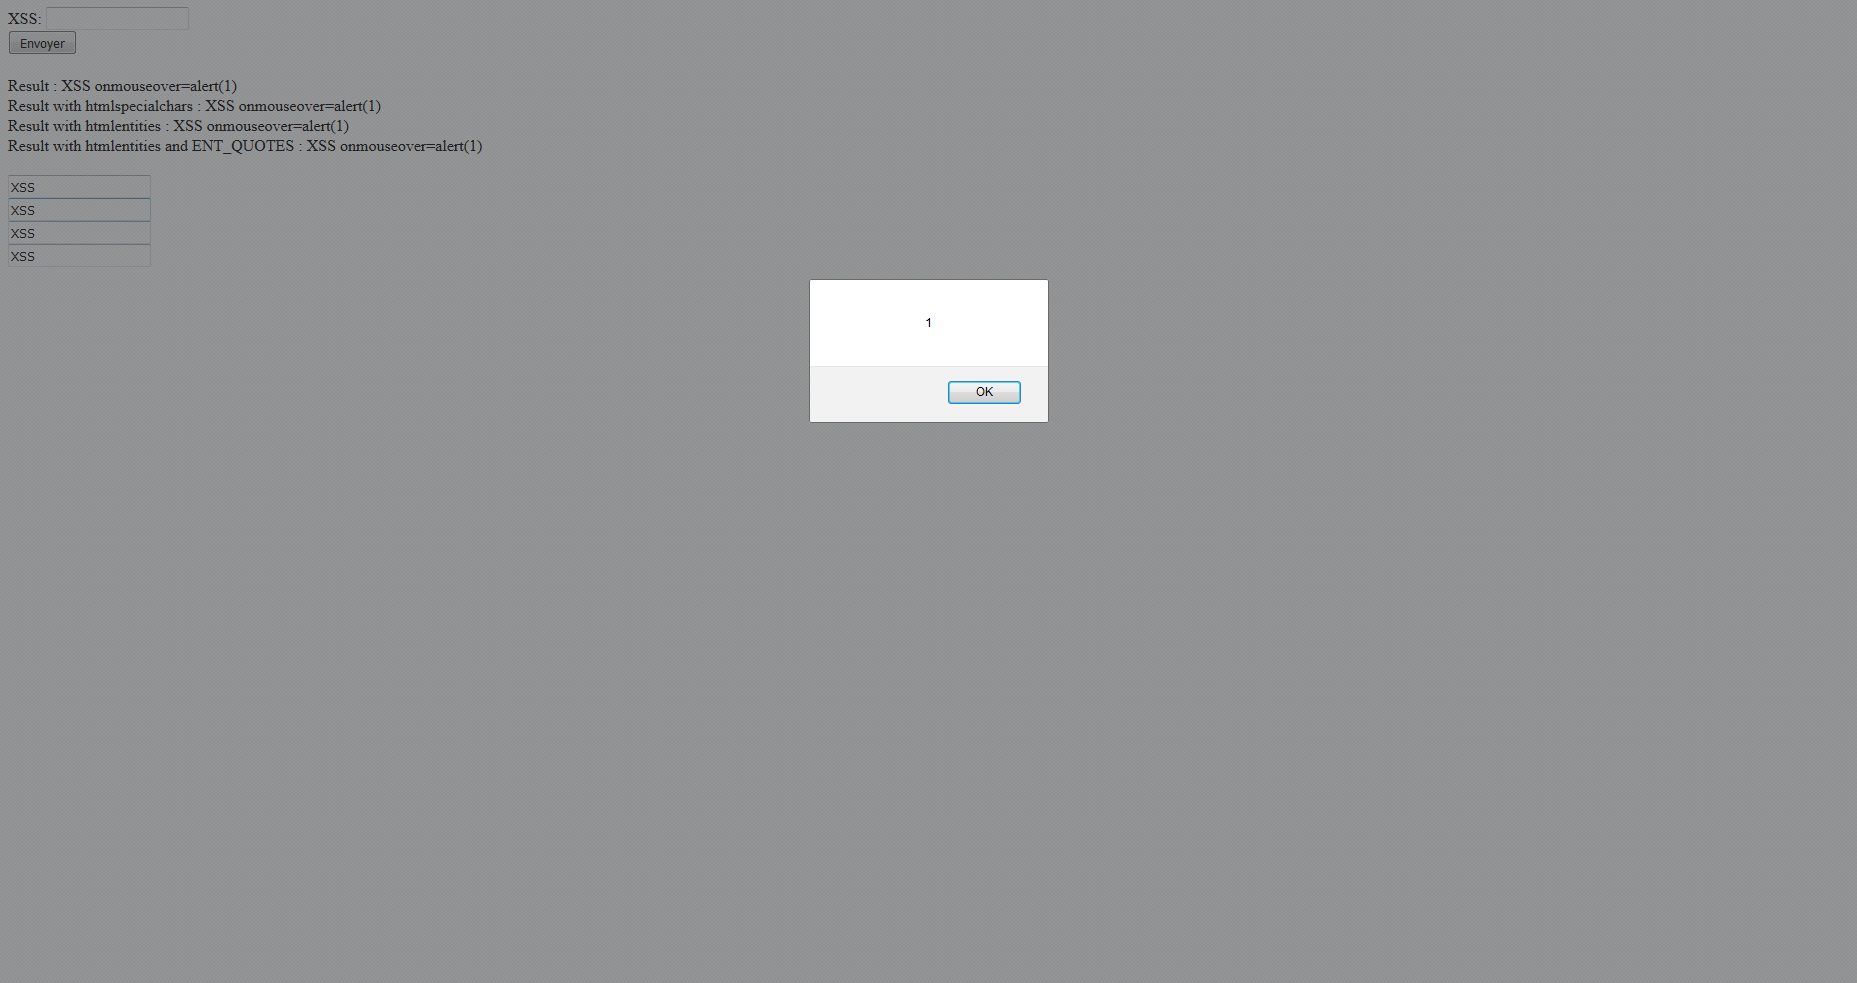
\includegraphics[width=\textwidth]{22}
}}
\vspace{0.2cm}

\vspace{0.2cm}
\subsection{XSS Trick avec UTF-7 - Bypass htmlspecialchars et htmlentities}

\subsection{XSS - Bypass htmlspecialchars et htmlentities avec les directives Javascript}

Comme dit plus haut, htmlspecialchars et htmlentities permettent seulement de convertir certains caractères et si l'on utilise aucun de ces caractères, ces deux fonctions deviennent inutiles. En utilisant les directives javascript, il est possible d'effectuer une XSS de la manière suivante :
\vspace{0.2cm}\\
\fbox{\parbox{\textwidth}{
javascript:alert('XSS')
}}
\vspace{0.2cm}

Prenons le script de test que j'utilise assez souvent depuis le début de cette section :
\vspace{0.2cm}\\
\fbox{\parbox{\textwidth}{
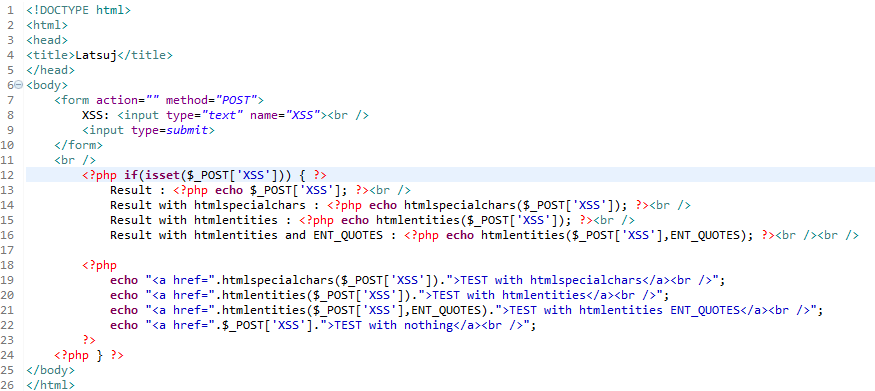
\includegraphics[width=\textwidth]{23}
}}
\vspace{0.2cm}

On obtient alors le résultat suivant :
\vspace{0.2cm}\\
\fbox{\parbox{\textwidth}{
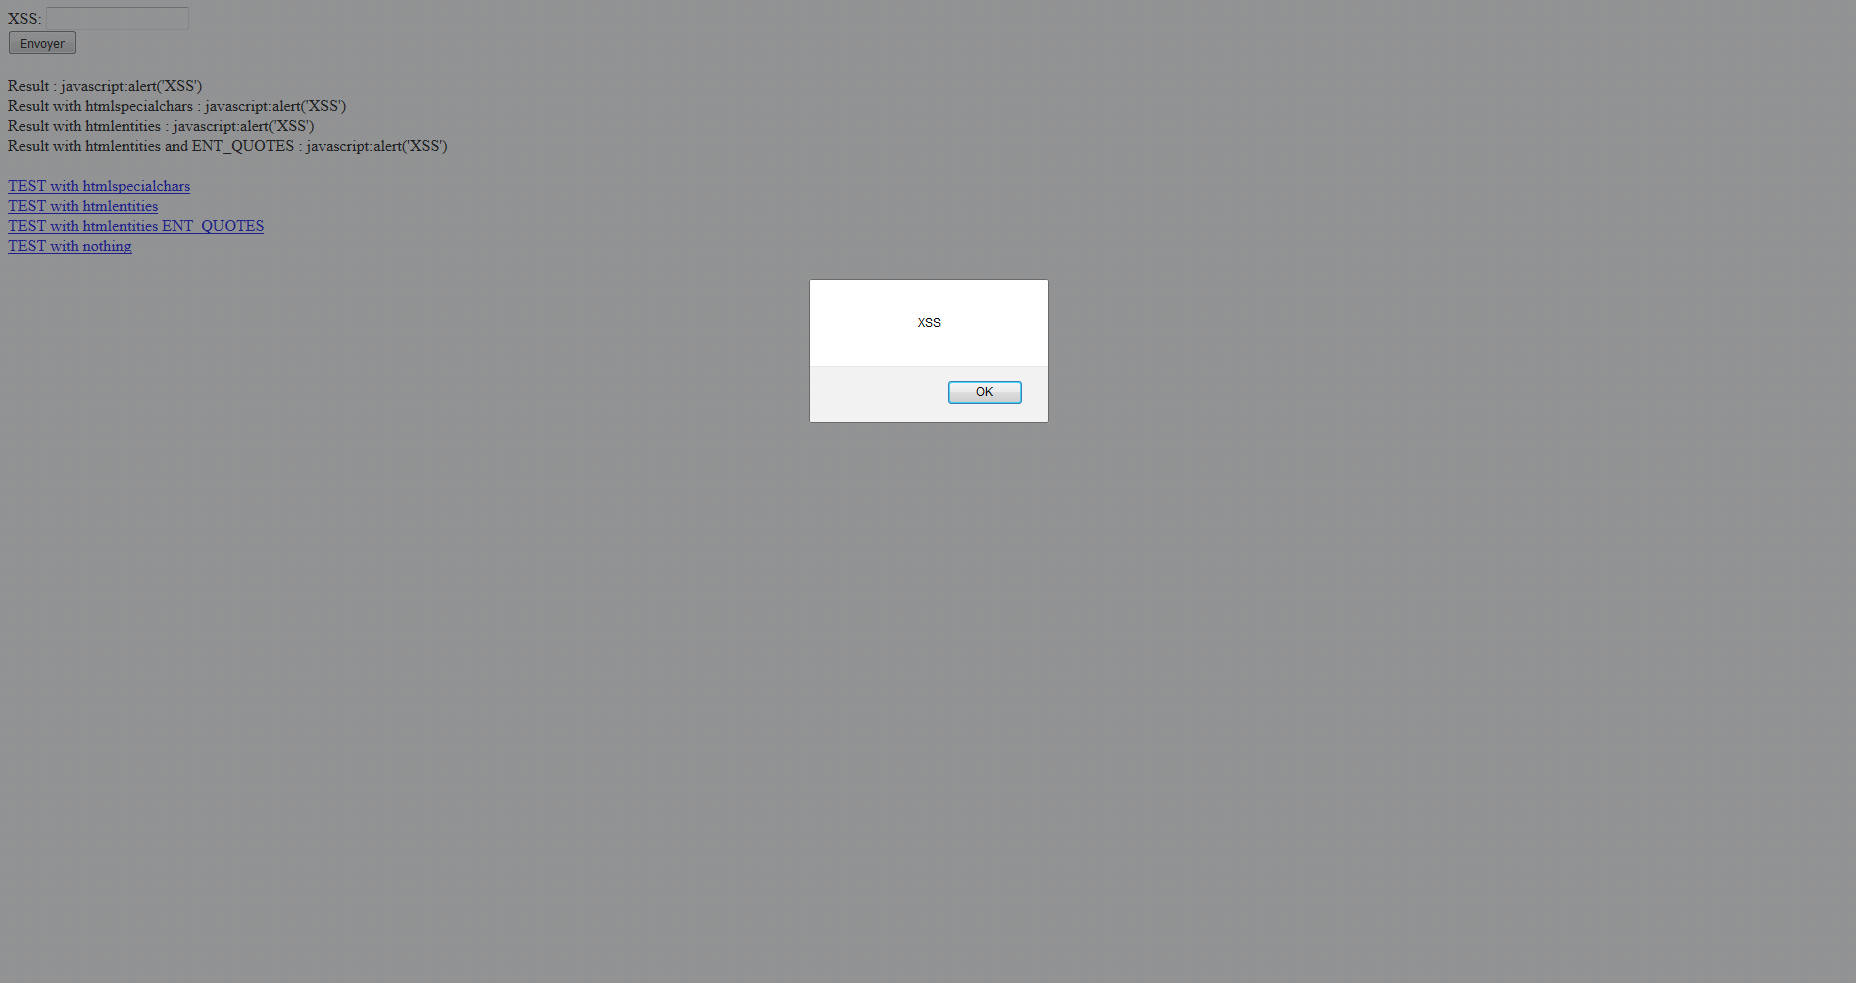
\includegraphics[width=\textwidth]{24}
}}
\vspace{0.2cm}

Comme on peut le voir, les deux fonctions sont complètement inutile contre ce type de script. Suivant la fonction utilisé, il est même possible de faire des redirections de pages et donc de faire ce que l'on veut (usurpation?).

\subsection{XSS - Bypass htmlspecialchars et htmlentities et les filtrages de chaines}

Sur plusieurs site, j'ai pu trouvé des chaines qui filtrait les directives javascripts en utilisant les fonctions suivantes : \textbf{strpos} ou encore \textbf{stripos}. Quand on regarde sur la documentation de PHP, on remarque que ces fonctions ne tiennent pas compte de la casse. Or on peux écrire la directive javascript sans tenir compte de la casse, c'est à dire que javascript:, Javascript:, JAVASCRIPT:, JaVaScRiPt: représente exactement la même chose. Je vais réutilisé l'exemple précédent en rajoutant un filtrage de chaines pour utilise la XSS suivante :
\vspace{0.2cm}\\
\fbox{\parbox{\textwidth}{
Javascript:alert(1)
}}
\vspace{0.2cm}

Le code de la page est le suivant. Il faut bien noté l'utilisation de la fonction strpos pour filtrer le mot javascript du résultat de l'input :
\vspace{0.2cm}\\
\fbox{\parbox{\textwidth}{
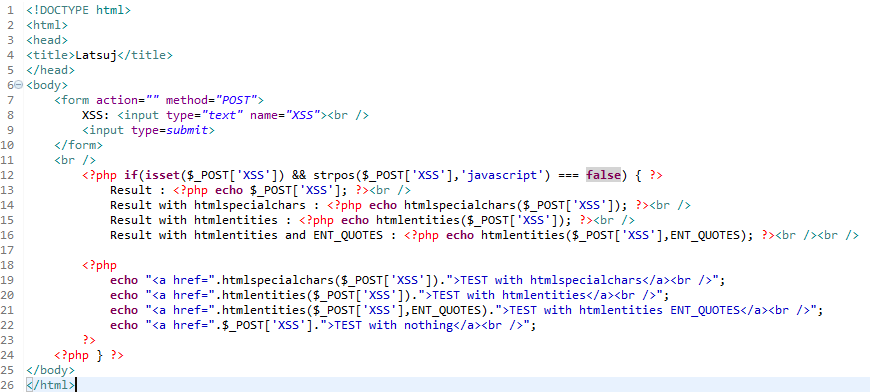
\includegraphics[width=\textwidth]{25}
}}
\vspace{0.2cm}

Et en utilisant la XSS, on bypass l'ensemble des fonctions :
\vspace{0.2cm}\\
\fbox{\parbox{\textwidth}{
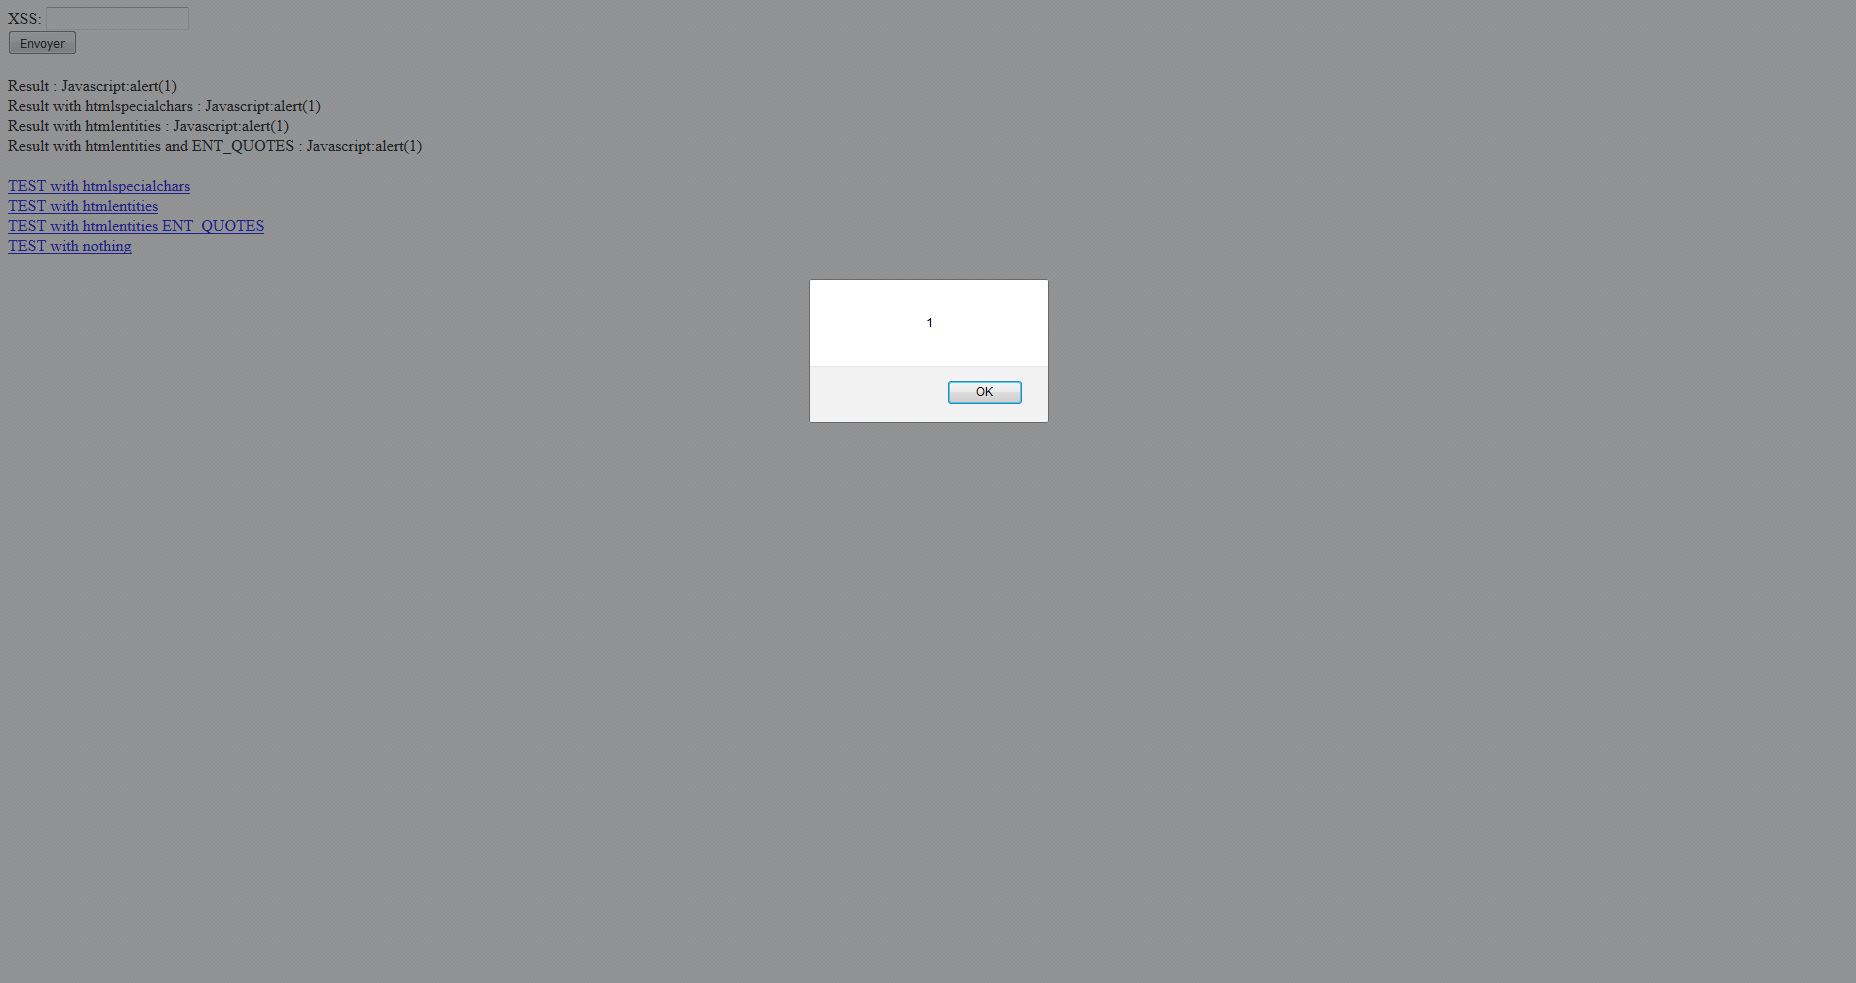
\includegraphics[width=\textwidth]{26}
}}
\vspace{0.2cm}

\subsection{XSS - Bypass htmlspecialchars et htmlentities avec les guillemets graves}

\newpage
\section{Bibliographie}
\subsection{SMTP Injection}
\begin{itemize}
\item http://www.phpsecure.info/v2/article/MailHeadersInject.php
\end{itemize}
\end{document}